\documentclass[12pt,a4paper]{article}
\usepackage[utf8]{inputenc}
\usepackage{graphicx}
\usepackage[frenchb]{babel}

\title{Snake}
\author{Antoine Forgerou \and Jérémy Bardon}
\date{}

\begin{document}

\maketitle
\tableofcontents

\newpage

\begin{abstract}
    Dans le cadre du module de logiciel extensible, nous avons développé 
    une plateforme à plugins basée sur la reflexion de java. 
    Pour illustrer le fonctionnement de cette plateforme, nous avons recréé 
    le célèbre jeu du snake.
\end{abstract} 

\section{Introduction}
Dans le cadre de notre projet, l'intérêt de développer le jeu du snake est double. 
Le premier avantage est que ce jeu est relativement simple, ce qui nous a permis de nous 
concentrer sur le développement de la plateforme sachant que nous sommes un groupe de 2 personnes
et non de 5. 
\\\\
Le second est que la plupart des composants du jeu peuvent être des plugins 
(affichage, map, score, etc ...) ce qui permet de mettre en avant l'utilisation 
de la plateforme.
    
\section{Plugin Principal}    
L'application est uniquement composée de plugins gérés par la plateforme. Le cœur 
de l'application est le plugin principal (executable par la plateforme) appelé \textbf{snakecore}. 
\\\\
Ce plugin est unique et gère le fonctionnement principal du snake. Il utilise 
des plugins secondaires respectant les besoins qu'il leurs impose à travers des 
interfaces.
\\\\
Lors du lancement, le jeu affiche une interface permettant soit de lancer le jeu, 
soit d'ouvrir une page de configuration qui permet de choisir les plugins à utiliser. 
Des plugins sont choisis par défaut afin que l'utilisateur puisse jouer directement. 

\begin{figure}[h]
    \centering
    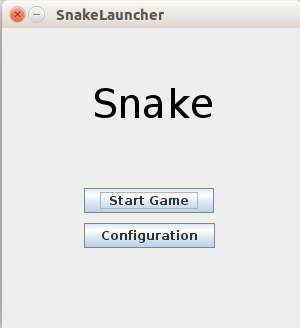
\includegraphics[scale=0.5]{ressources/menu.png}
    \caption{Menu du Snake}
\end{figure}    

\newpage
Dans l'interface de configuration des plugins, ces derniers sont triés par types. 
Lorsque plusieurs plugins sont disponibles pour un type il est possible d'en 
utiliser plusieurs si cela est précisé. Certains types de plugins sont obligatoires
mais il en existe d'autres qui sont facultatifs.

\begin{figure}[h]
    \centering
    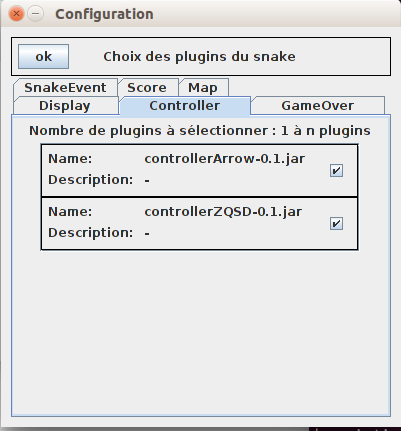
\includegraphics[scale=0.4]{ressources/configurationControler.png}
    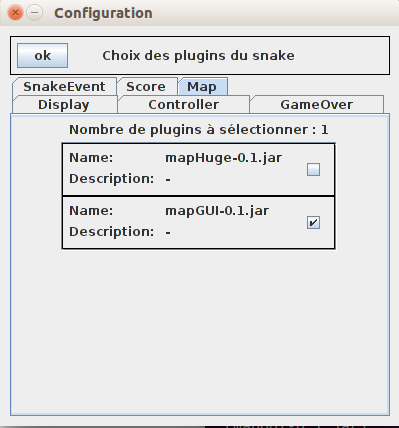
\includegraphics[scale=0.4]{ressources/configurationMap.png}
    \caption{Interface de configuration - Controler / Map}
\end{figure}       
    
Quand le jeu est lancé, le plugin principal demande à la plateforme de charger 
la liste des plugins séléctionnés afin de pouvoir les utiliser. Une fois les 
plugins secondaires chargés, le jeu du snake est lancé dans une autre fenêtre et
s'arrête lorsque le joueur à perdu (cet aspect est un plugin).

\begin{figure}[h]
    \centering
    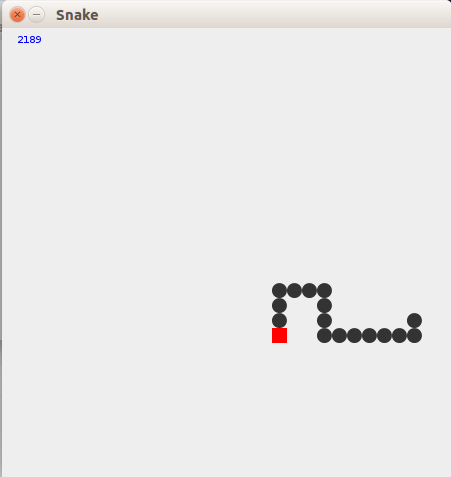
\includegraphics[scale=0.4]{ressources/snake.png}
    \caption{Une partie de Snake}
\end{figure}   
    
\section{Plugins Secondaires}    
Ce projet utilise notre plateforme à plugins le plus possible afin de déléguer 
l'implémentation de certaines parties du jeu. 
\\\\
Le plugin principal défini les interfaces dont il a besoin ou qu'il supporte et c'est 
ce qui va servir de base pour obliger les plugins secondaire à implémenter
certaines fonctionnalités qui sont requises par le core. 
\\\\
Les plugins secondaires peuvent être classés en plusieurs catégories. En effet 
certains sont essentiels au bon fonctionnement du programme alors que d'autres 
sont optionnels. De plus, le core peut -- pour certaines catégories de plugins -- 
utiliser en parallèle plusieurs plugins secondaires d'un même type. 
    
\subsection{Interface graphique}
La fenêtre en jeu que va afficher le plugin principal est lui-même un plugin. 
En effet, il est possible d'imaginer plusieurs interfaces graphiques différentes mais
il reste nécessaire au fonctionnement du programme. 
\\\\
Le core ne peut pas lancer plusieurs interfaces car nous souhaitons garder
une seule interface pour représenter le jeu à un moment donné.
    
\subsection{Terrain de jeu}
Ce type de plugin représente la map sur laquelle le jeu se déroule. 
Il permet de fixer la taille de la carte mais aussi elle contient aussi 
tout les éléments qui sont dessus: serpent et grenouilles.
\\\\
Pour une partie donnée, il ne peut y avoir qu'une map, ce type de plugin est donc 
unique.
    
\subsection{Contrôle du serpent}
Le principe du jeu est de manger les grenouilles, par conséquent il nécessaire
de pouvoir changer la direction du serpent (qui avance tout droit).
\\\\
Ce plugin a accès au serpent et il peut donc changer sa direction lorsqu'il
capte un événement clavier. 
Le type Controlleur est nécessaire au bon fonctionnement, car il est impossible 
de jouer sans. 
\\\\
Nous avons choisi de permettre au joueur de pouvoir jouer avec plusieurs 
controlleurs simultanément, cette option n'entravant pas le bon 
fonctionnement du jeu.  
       
\subsection{Game over}
Ce qui ce passe après la défaite du joueur -- par défaut contact du serpent avec lui 
même ou avec un mur -- est géré par un type de plugin. À travers ce plugin
il est possible de modifier les conditions et les comportements de la défaite. 
\\\\
Ce type de plugin est nécessaire pour pouvoir gérer la défaite du joueur sinon 
le jeu ne s'arrêtera pas. Il constitue un point d'extension très fort du programme puisque
l'on peut imaginer beaucoup de modes de jeux sachant que l'on à accès à des informations
comme le score et le temps passé.

\subsection{Évolution de l'environnement} 
Nous avons souhaiter gérer l'évolution de l'environnement de jeu au cours de 
la partie.
\\\\
Le but de ce plugin à événements est de pouvoir changer certains élément du jeu 
au cours de la partie lorsque certaines actions sont effectués. Ce type de plugin 
est optionnel mais peut aussi être multiple. 
\\\\
Exemple de plugins développés: 
\begin{itemize}
   \item Augmentation de la vitesse de jeu à chaque tour
   \item Le snake grandi plus ou moins vite lorsqu'il mange une grenouille    
\end{itemize}
\end{document}
